\section{Bioinformatics}
\label{sec:bioinfo}

Bioinformatics is a field applying computational methods for addressing biological challenges.
This is of especial interest in areas where the amount of biological data is so large that other means of processing the data is infeasible.
One prominent area of biology where this is the case is sequence analysis, where huge amounts of DNA sequences are analyzed to understand biological phenomena or make useful predictions.

In this section we study such a bioinformatics application, called T-CUP~\cite{DybowskiHeHo2010}, concerned with predicting the resistance of a patient to certain types of \HIV drugs.
T-CUP uses machine learning as a statistical method to build a model based on millions of analyzed DNA sequences.
Based on this model the software can predict the resistance of a patient to a particular type of \HIV drugs which is of obvious practical use when determine which drugs to use for treating the patient.
T-CUP is designed to replace an expensive and time-consuming blood analysis which is currently used.

\subsection*{Biological Background}
There exists three classes of \HIV viruses, called R5, X4 and X4R5.
The names relate to the co-receptors the virus uses to connect to the host cell it infects:
the R5 virus uses the {\small CCR5} co-receptor, the X4 virus the {\small CXCR4} co-receptor, and the X4R5 virus uses both.
\autoref{fig:hiv} shows a cell with the co-receptors.
\begin{figure}[t]
  \centering
  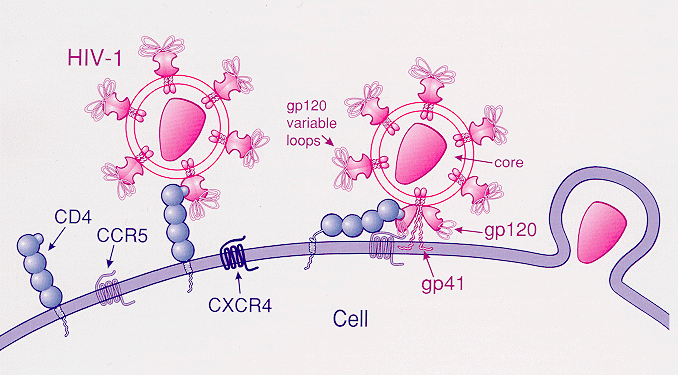
\includegraphics[width=.85\textwidth]{HIV.png}
  \caption[]%
          {}
  \label{fig:hiv}
\end{figure}
Certain HIV drugs work by blocking the {\small CCR5} co-receptor and, thus, make it unavailable for the HIV virus.
Obviously, these drugs are only effective against the R5 and X4R5 types of the HIV virus.
It is, therefore, of interest when choosing the appropriate drug for treating a patient with which type of HIV virus the patient is infected.
There exists a blood test which can be used to determine the HIV virus type.
Unfortunately is this test expensive and time-consuming, so that often the treatment starts before the results of the test are known.

\subsection*{T-CUP}
The T-CUP software attempts to predict the type of the HIV virus from analyzing a large amount of DNA sequences.
Using \emph{next-generation sequencing} ({\small NGS}) millions or even billions of reads of DNA sequences can be obtained from a single sample.
This large number of reads require substantial computational power to be processed ans analyzed.

The existing T-CUP software was implemented using the statistical language R which has an easy to use interface for statistics tasks and offers a rich ecosystem of packages concerned with typical bioinformatics challenges.
Unfortunately, R is an interpreted language lacking of execution speed compared to statically compiled languages like C.
The original R implementation of T-CUP was able to process 9 DNA sequences per seconds making the processing a millions of DNA sequences infeasible.
By rewriting the core computational part in C one can obtain a large performance improvement processing about 4000 DNA sequences per seconds and, thus, bringing the runtime from months and weeks down to hours.
We will discuss in the following how we can further reduce the runtime to a matter of minutes by parallelizing the application.

Fortunately, most of the T-CUP software can be fairly easily parallelized as each individual sequence can be analyzed largely independently.
\autoref{fig:tcup} shows an overview of the steps performed by T-CUP.
\begin{figure}
  \centering
  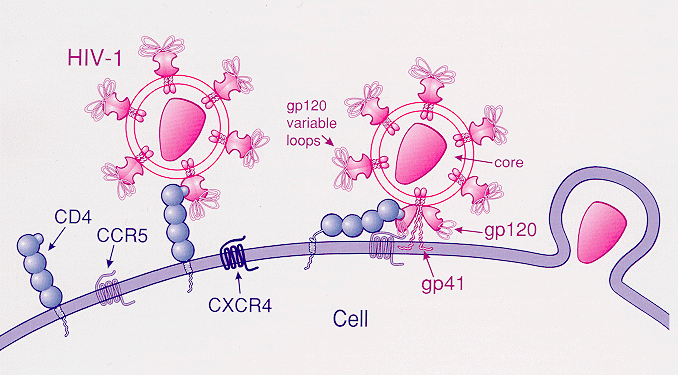
\includegraphics[width=.85\textwidth]{HIV.png}
  \caption[]%
          {}
  \label{fig:tcup}
\end{figure}
We will focus our discussion on the four most time-consuming steps comprising more than 75\% of the overall runtime of the application.
These steps are: alignment, translation, ESP computation, and classification.

\paragraph{Alignment}
In the alignment step all processed DNA sequences are aligned against a reference sequence to find the section of each DNA sequence we are interested in.
The Needleman-Wunsch algorithm~\cite{} is a widely used algorithm for aligning two sequences.
To perform the alignment both sequences are arranged on the columns and rows of a matrix as shown in \autoref{fig:needlemanWunsch}.
The algorithm computes each entry in the matrix following

\subsection*{\SkelCL implementation}

\subsection*{Programming effort}

\subsection*{Performance experiments}

